\section{良いアルゴリズム,わるいアルゴリズム}
\subsection{アルゴリズムとは}
\begin{frame}[containsverbatim, shrink]
\frametitle{アルゴリズム}
  \begin{itemize}
\item 前回まで再帰関数についてお話しました
\item これはアルゴリズム的に計算可能という概念を定義する上で重要な役割をします
\item 関数 \(f:D^n\rightarrow D\) が計算可能とは,それを計算するアルゴリズム(算法)が存在すること
    \begin{itemize}
\item アルゴリズムとは停止する命令の有限の列をいう
\item コンピュータにプログラムできるなにがしか
    \end{itemize}
\item たとえば,
    \begin{itemize}
\item $D$ は最小(あるは極小)があって並んでいるという構造を持つ
\item \(x\in D\) として \(f(x)=G(f\upharpoonright x)\)
\item $D$ を自然数すれば \((N;0,S,+,-,\times,\div,\mathrm{mod},<)\)
\item 計算を \(0,S,+,-,\times,\div,\mathrm{mod},<\) を再帰や合成で列として構成
    \end{itemize}
\item 別の方法として Turing machine を紹介(ホワイトボードに書きます)
\item 計算可能な関数のクラスも理論的に興味深いが,それは別の機会
  \end{itemize}
\end{frame}
\begin{frame}
\frametitle{良いアルゴリズム}
  \begin{itemize}
\item ここでは,すでに計算可能な関数のクラスがあって,その計算の複雑さについて議論する
\item 計算のやり方には良い方法とわるい方法がある
\item 良い方法というのは少ない計算で目的の値を求めること
\item 良い悪いの尺度のひとつ時間計算量について見ていく
\item \(0,S,+,-,\times,\div,\mathrm{mod},<\) のような演算が何回必要かを測る
\item 単にプログラムが動けばいいでなくて
  \end{itemize}
\end{frame}
\subsection{最大公約数を例に導入}
\begin{frame}
\frametitle{まずは最大公約数}
  \begin{itemize}
\item 関数 GCD をふたつの自然数の公約数のうち最大のもの
\item アルゴリズムでは具体的に最大公約数をもとめる計算の仕方を議論する
\item 計算の仕方はいくつか考えられる
    \begin{itemize}
\item アルゴリズムの書き方も自然言語で書いたりいろいろ
    \end{itemize}
  \end{itemize}
  \begin{columns}[t]
    \begin{column}{0.5\textwidth}
      \begin{block}{素朴な方法}
ふたつの整数 \(x, y\) について $1$ から順に \(\min(x,y)\) まで
割って,割り切れる最大の整数
      \end{block}
    \end{column}
    \begin{column}{0.5\textwidth}
      \begin{block}{ユーグリッドの互除法}
\scriptsize
\(x_1, x_2\) の最大公約数は $x_1$ を $x_2$ で割ったときの剰余と $x_2$ の最大公約数に等しい
%\setlength{\abovedisplayskip}{10pt}
        \begin{displaymath}
          \begin{array}{rcl}
x_1 &=& n_1 x_2 + x_3\\
x_2 &=& n_2 x_3 + x_4\\
x_3 &=& n_3 x_4 + x_5\\
&\vdots&
          \end{array}
        \end{displaymath}
      \end{block}
    \end{column}
  \end{columns}
\end{frame}
\begin{frame}[fragile,shrink]
\frametitle{最大公約数 (Greatest Common Divisor) のプログラム}
  \begin{itemize}
\item それぞれの実行時間を比較するので見ていてください
    \begin{itemize}
\item 適当な数字思いつかないので
\item 10000000 と 10203040 の最大公約数
\item 62979284285501 と 62873258567731 の最大公約数
    \end{itemize}
  \end{itemize}
  \begin{columns}[t]
    \begin{column}{0.45\textwidth}
      \begin{lstlisting}[caption={gcd.py}]
def gcd(x,y):
  def min(x,y):
    if (x>y):
      return y
    else:
      return x
  gcm=1
  n=min(x,y)
  for i in range(1,n+1):
    if (x%i==0) and (y%i==0):
      gcm=i
  return (gcm)
      \end{lstlisting}
    \end{column}
    \begin{column}{0.45\textwidth}
      \begin{lstlisting}[caption={gcd.py},label=lst:euclid]
def euclid1(x1,x2):
  if x2==0:
    return (x1)
  else:
    return (euclid1(x2,x1%x2))
def euclid(x1,x2):
  def swap(x1,x2):
    return x2,x1
  if (x1<x2) :
    x1,x2 = swap(x1,x2)
  return(euclid1(x1,x2))
      \end{lstlisting}
    \end{column}
  \end{columns}
\end{frame}
\begin{frame}[fragile]
\frametitle{実行時間の違いについての考察}
  \begin{itemize}
\item Naive な方法
    \begin{itemize}
\item mod や比較の回数を数えてみる
\item $n$ 回で $n$ は $x$ か $y$ の小さい方になっている
    \end{itemize}
\item ユーグリッドの互除法
    \begin{itemize}
\item $n$ よりは少ない回数で計算できる
    \end{itemize}
  \end{itemize}
  \begin{columns}[t]
    \begin{column}{0.45\textwidth}
      \begin{itembox}{euclid(32204,14744)}
\scriptsize
        \begin{verbatim}
  euculid(32204,14744)
=>euclid1(14744,2656)
=>euclid1(2656,1162)
=>euclid1(1162,332)
=>euclid1(332,166)
=>euclid1(166,0)
=>166
        \end{verbatim}
      \end{itembox}
    \end{column}
    \begin{column}{0.45\textwidth}
      \begin{itembox}{euclid(34,21)}
\scriptsize
        \begin{verbatim}
  euculid(34,21)
=>euclid1(21,13)
=>euclid1(13,8)
=>euclid1(8,5)
=>euclid1(5,3)
=>euclid1(3,2)
=>euclid1(2,1)
=>euclid1(1,0)
=>1
        \end{verbatim}
      \end{itembox}
    \end{column}
  \end{columns}
\end{frame}
\begin{frame}[fragile]
\frametitle{ユーグリッドの互除法の演算回数の見積もり}
  \begin{itemize}
\item 最悪の場合について考える
\item 割り算の商がいつまでも 1 であるとき最悪になる
\item となり合う 2 つの Fibonacci 数のとき最悪になる
\item 下の図で $q_i=1$ for \(1\le i\le n-1\) としたとき Fibonacci 数 \(1,1,2,3,5,8,13,21,\ldots\) を逆にたどったもの
  \end{itemize}
  \begin{columns}[t]
    \begin{column}{0.45\textwidth}
\centering
      \begin{math}
        \begin{array}{rcl}
r_0 &=& q_1 r_1 + r_2\\
r_1 &=& q_2 r_2 + r_3\\
r_2 &=& q_3 r_3 + r_4\\
&\vdots&\\
r_{n-2} &=& q_{n-1}r_{n-1} + r_{n}\\
r_{n-1} &=& q_{n}r_{n}\\
&&\mbox{where } r_0=x_1>r_1=x_2
        \end{array}
      \end{math}
    \end{column}
    \begin{column}{0.45\textwidth}
\centering
      \begin{math}
        \begin{array}{rcl}
21 &=& 13 + 8\\
13 &=& 8 + 5\\
 8 &=& 5 + 3\\
 5 &=& 3 + 2\\
 3 &=& 2 + 1\\
 2 &=& 2 \cdot 1
        \end{array}
      \end{math}
    \end{column}
  \end{columns}
\end{frame}
\newcommand{\fib}{\mathop{\mathrm{fib}}\nolimits}
\begin{frame}[fragile,shrink]
\frametitle{ユーグリッドの互除法の演算回数}
  \begin{itemize}
\item \(r_1>r_2>\ldots>r_{n-1}>r_n>r_{n+1}=0\)
\item 小さい方の数 \(r_1\)は \(n+1\) 番目の Fibonacci 数 \(f_{n+1}\) であるかそれより大きい
  \end{itemize}
  \begin{columns}[t]
    \begin{column}{0.45\textwidth}
\centering
      \begin{math}
        \begin{array}{rcl}
r_0 &=& r_1 + r_2\\
r_1 &=& r_2 + r_3\\
r_2 &=& r_3 + r_4\\
&\vdots&\\
r_{n-2} &=& r_{n-1} + r_{n}\\
r_{n-1} &=& q_{n}r_{n}\\
         && (q_n\ge 2)
        \end{array}
      \end{math}
    \end{column}
    \begin{column}{0.45\textwidth}
\centering
      \begin{math}
        \begin{array}{rcl}
r_n     &\ge& 1(=f_2)\\
r_{n-1} &\ge& 2(=f_3)\\
r_{n-2} &\ge& f_3+f_2(=f_4)\\
 &\vdots& \\
 r_{n-(l-1)}&\ge& f_l+f_{l-1}\\
 &\vdots& \\
r_{2} &\ge& f_{n-1}+f_{n-2}(=f_n)\\
r_{1} &\ge& f_n+f_{n-1}(=f_{n+1})\\
        \end{array}
      \end{math}
    \end{column}
  \end{columns}
\end{frame}
\begin{frame}[fragile,shrink]
\frametitle{ユーグリッドの互除法の演算回数\textemdash つづき}
  \begin{itemize}
\item $r_1=N$ として,このことから
  \end{itemize}
  \begin{center}  
    \begin{math}
      \begin{array}{rcll}
N&\ge& f_{n+1}\\
N&\ge& \phi^{n-1}&(\mbox{by }f_{n+1}>\phi^{n-1} \mbox{ for }n>2\\
                &&&\mbox{where }\phi=\frac{(1+\sqrt{5})}{2})\\
\log_{10}N&\ge&(n-1)\log_{10}\phi\\
\log_{10}N&\ge&(n-1)\log_{10}\phi>\frac{n-1}{5}\\
n&<&5\cdot\log_{10}N+1\\
      \end{array}
    \end{math}
  \end{center}
  \begin{itemize}
\item Naive な方法の演算回数 N 回 よりは少ない
  \end{itemize}
\end{frame}
\subsection{べき乗のアルゴリズム}
\begin{frame}[fragile,shrink]
\frametitle{Quiz2: べき乗 (Power) の計算}
  \begin{itemize}
\item 下の例を参考にべき乗を求める良いアルゴリズムを考えてみてください
\item \(b^8\) を求めるのに乗算を 8 回と 3 回
\item  8 回より 3 回の方が良い子
\item power-skeleton.py が\href{https://sites.google.com/presystems.xyz/elementaryCS/}{\beamerbutton{https://sites.google.com/presystems.xyz/elementaryCS/}} に置いてあるので,
ループに変更して実行時間を比較してみてください
\item 提出はいつもの T2Schola からソースコードを提出
  \end{itemize}
  \begin{example}[\(b^8\) の計算]
  \begin{columns}[t]
    \begin{column}{0.55\textwidth}
\(b\times(b\times(b\times(b\times(b\times(b\times(b\times b))))))\)
    \end{column}
    \begin{column}{0.35\textwidth}
\centering
      \begin{math}
        \begin{array}{rcl}
b^2 &=& b \times b\\
b^4 &=& b^2 \times b^2\\
b^8 &=& b^4 \times b^4
        \end{array}
      \end{math}
    \end{column}
  \end{columns}
  \end{example}
\end{frame}
\begin{frame}[fragile,shrink]
\frametitle{べき乗 (Power) のヒント}
  \begin{itemize}
\item 指数は偶数のとき半分に,奇数のとき $-1$ 減る
  \end{itemize}
  \begin{columns}
    \begin{column}{0.45\textwidth}
      \begin{math}
        \begin{array}{rcl}
b^n &=& (b^{\frac{n}{2}})^{2}\\
&& n \mbox{が偶数のとき}\\
b^n &=& b \times b^{n-1}\\
&& n \mbox{が奇数のとき}
        \end{array}
      \end{math}
    \end{column}
    \begin{column}{0.5\textwidth}
      \begin{lstlisting}[caption={power.py},label=fast_power]
def fast_power(b,n):
  def square(x):
    return(x*x)
  def is_even(n):
    if (n%2==0):
      return(True)
    else:
      return(False)
  if (n==1):
    return(b) 
  else:
    if (is_even(n)):
      return(square(fast_power(b,n/2)))
    else:
      return((b*fast_power(b,n-1)))
      \end{lstlisting}
    \end{column}
  \end{columns}
\end{frame}
\section{時間計算量}
\subsection{Big\textendash O Notation}
\begin{frame}[shrink]
\frametitle{時間計算量}
  \begin{itemize}
\item アルゴリズムの良し悪しを測る尺度についてみていきます
\item 良し悪しの基準
    \begin{itemize}
\item 良いアルゴリズム,わるいアルゴリズムを実行時間を計測して比較
\item 入力に対し結果を得るまでの演算 (四則演算や比較演算) の実行回数を見積もって比較
    \end{itemize}
\item 実行時間は CPU や演算の実現方式に依存し計算しようとすると複雑な式になってしまう
\item 演算回数 (時間計算量という)をもとに単純な式で見積もることにする
    \begin{itemize}
\item CPU や実現方式といったものは無視
    \end{itemize}
\item 実行時間がどう変化するかの傾向を見積もれれば十分
  \end{itemize}
  \begin{example}
入力サイズ $n$ として一方は \(n^2\) ,もう一方は \(n^3\) 回演算を行うとすれば,
 $n$ が十分に大きいときには前者の方が良い
  \end{example}
\end{frame}
\begin{frame}[shrink]
\frametitle{Big\textendash$O$ 記法}
  \begin{itemize}
\item $n$ を入力のサイズとして,演算回数 \(f(n)\) で傾向をつかむ
  \end{itemize}
  \begin{definition}
2 つの関数 \(f, g\colon N\rightarrow R^{>0}\) とする.
    \begin{center}
\(\forall n>k\colon f(n)\leq c\cdot g(n)\)
    \end{center}
となるような \(c, k\) が存在するならば \(f(n)\Rightarrow O(g(n))\) とする
  \end{definition}
  \begin{example}
\(f(n)=n^2+2n+1\) は,たとえば \(c=4, k=1\) として \(g(n)=n^2\),よって \(f(n)\) は \(O(n^2)\) となる.
  \end{example}
\end{frame}
\begin{frame}[shrink]
\frametitle{\(f(n)=n^2+2n+1\) は \(O(n^2)\)}
  \begin{itemize}
\item \(n>1\)(=\(k\)) で \(2n\leq 2n^2, 1\leq n^2\) なので
    \begin{displaymath}
0\leq n^2+2n+1\leq n^2+2n^2+n^2= 4n^2
    \end{displaymath}
\item \(c=4, k=1, g(n)=n^2\) として,
\item \(f(n)=n^2+2n+1<4\cdot n^2\)\ \textemdash\{\(f(n)\leq c\cdot g(n)\)\}
\item \(n\geq 2\) とすると \(2n<n^2, 1<n^2\) 
    \begin{displaymath}
0\leq n^2+2n+1\leq n^2+n^2+n^2= 3n^2
    \end{displaymath}
  \end{itemize}
  \begin{center}
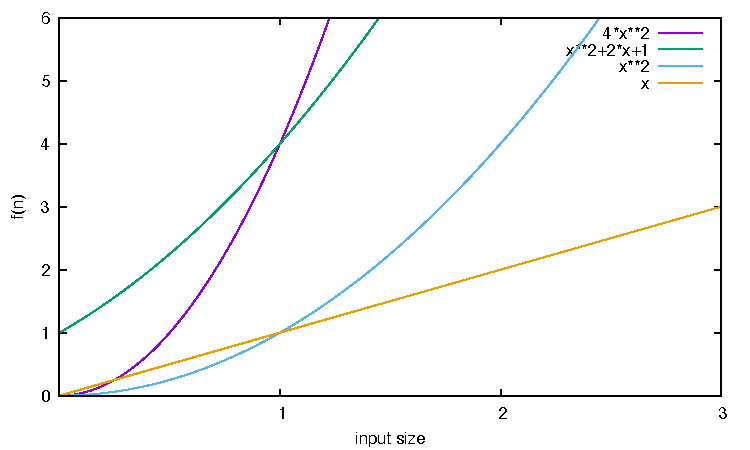
\includegraphics[scale=0.6]{./progs/witness.pdf}
  \end{center}
\end{frame}
\begin{frame}[shrink]
\frametitle{ユーグリットの互除法とべき乗のアルゴリズムのオーダ}
  \begin{example}[ユーグリットの互除法]
    \begin{itemize}
\item Lame の定理: 割り算の回数は,小さい数 $n$ の桁数の 5 倍以下である
    \end{itemize}
よって,\(\forall n\ge 10:(5(\log_{10}n)+1<(5+1)\log_{10} n)\Rightarrow O(\log n)\)
  \end{example}
  \begin{example}[べき乗]
    \begin{itemize}
\item 指数を $n$,2 進表記の 1 の数 $j$,偶数のときはいつも半分になるので $m$ 回偶数が出現するとして,
    \end{itemize}
    \begin{center}
      \begin{math}
        \begin{array}{rcl}
n&=&2^m\\
\log_2 n &=& m
        \end{array}
      \end{math}
    \end{center}
よって, \(\forall n\ge2:((\log_2 n)+(j-1)<(1+(j-1))\log_2 n)\Rightarrow O(\log n)\).
  \end{example}
\end{frame}
\begin{frame}[containsverbatim,shrink]
\frametitle{べき乗 (Power) の演算回数の見積もり}
  \begin{itemize}
\scriptsize
\item 各繰り返しで掛け算の回数は 1 回
\item 偶数は何回出てくるか,奇数は何回出てくるかを数える
\item $n$ を指数, $m$ を\(\frac{1}{2}\) する回数として \(\frac{n}{2^m}=1\)
\item そのうち,何回奇数が出てくるかは $n$ を二進表記した時の 1 の数による
    \begin{itemize}
\scriptsize
\item \(\frac{1}{2}\) するとは右に 1 ビットシフト
\item 最下位ビットが 1 のとき奇数
\item 最後 0 乗は計算しないので(1 の数)-1
    \end{itemize}
\item \(\lfloor\log_2 1000\rfloor+5\)=14 回
  \end{itemize}
  \begin{columns}
    \begin{column}{0.45\textwidth}
      \begin{block}{偶数の出現回数}
        \begin{math}
          \begin{array}{c}
\frac{n}{2^m}=1\\
n=2^m\\
\lfloor\log_2 n\rfloor = m
          \end{array}
        \end{math}
      \end{block}
    \end{column}
    \begin{column}{0.5\textwidth}
      \begin{block}{奇数の出現回数}
\scriptsize
        \begin{math}
          \begin{array}{cl}
(1000)_{10}=&(1111101000)_{2}\\
&\Rightarrow_{\frac{1}{2}}0111110100\\
&\Rightarrow_{\frac{1}{2}}0011111010\\
&\Rightarrow_{\frac{1}{2}}0000111101\\
&\Rightarrow_{-1}0000111100\\
&\Rightarrow_{\frac{1}{2}}0000011110\\
&\cdots\\
&\Rightarrow_{\frac{1}{2}}0000000001
          \end{array}
        \end{math}
      \end{block}
    \end{column}
  \end{columns}
\end{frame}
%\begin{frame}[shrink]
%\frametitle{Big\textendash$\Omega$}
%  \begin{itemize}
%\item Big\textendash$O$ は,``それより大きくなることはない''ということ
%\item では``それより小さくなることはない''ということは ?
%  \end{itemize}
%  \begin{definition}
%2 つの関数 \(f, g\colon N\rightarrow R^{>0}\) とする.
%    \begin{center}
%\(\forall n>k\colon f(n)\geq c\cdot g(n)\)
%    \end{center}
%となるような \(c, k\) が存在するならば \(f(n)=\Omega(g(n))\) とする
%  \end{definition}
%  \begin{block}{オーダ (order)}
%    \begin{itemize}
%\item \(f(n)=O(g(n))\) かつ \(f(n)=\Omega(g(n))\) のとき \(f(n)\) は オーダ \(g(n)\) という
%\item あるいは \(f(n)=O(g(n))\) かつ \(g(n)=O(f(n))\) のとき
%\item e.g. \(n^2+2n+1=O(n^2)\) で \(n^2=O(n^2+2n+1)\) である
%    \end{itemize}
%  \end{block}
%\end{frame}
\section{Sorting}
\subsection{各種ソートアルゴリズム}
\begin{frame}[shrink]
\frametitle{Sorting}
  \begin{itemize}
\item Sorting は 2 つの要素の比較と入れ替えだけを用いて,
与えられた集合の要素のリストを昇順(降順)に並べたリストを作ること
\item 例えば \{3,2,4,1,5\} と与えられていれば \{1,2,3,4,5\} と並べたリストを作成する
\item データベースシステムなど多くの場面で利用されている
\item 多くのアルゴリズムが提案されている
\item ここではバブルソート (bubble sort),挿入ソート (insertion sort),クイックソート (quick sort) を例に機械的にアルゴリズムから計算量を求めていく方法を見てみる
  \end{itemize}
\end{frame}
\begin{frame}[containsverbatim,shrink]
\frametitle{Bubble Sort}
  \begin{columns}[t,onlytextwidth]
    \begin{column}{0.5\linewidth}
      \begin{lstlisting}[caption={擬似コード},label=bubble_sort]
def bubble_sort(numbers):
  for i in {1..n-1}:
    for j in {n..i+1}:
      if (numbers[j]<numbers[j-1]):
        numbers[j],numbers[j-1]を入替え
  return(numbers)  
      \end{lstlisting}
      \begin{itembox}[l]{計算量}
        \begin{itemize}
\tiny
\item 配列のサイズを $n$ として
\item 4-5 行は入力サイズによらず一定; $c$
\item 3-6 行の演算回数は各繰り返しの演算回数の和; $c$ を \(n-i\) 回繰り返すので \(c(n-i)\)
\item 2-6 行の演算回数は各繰り返しで \(c(n-i)\) を \((n-1)\) 回繰り返すので
\item 全体で \(\sum_{i=1}^{n-1} c(n-i)=\frac{cn(n-1)}{2}=c(\frac{n^2}{2}-\frac{n}{2})\)
        \end{itemize}
      \end{itembox}
    \end{column}
    \begin{column}{0.55\linewidth}{様相}
      \begin{center}
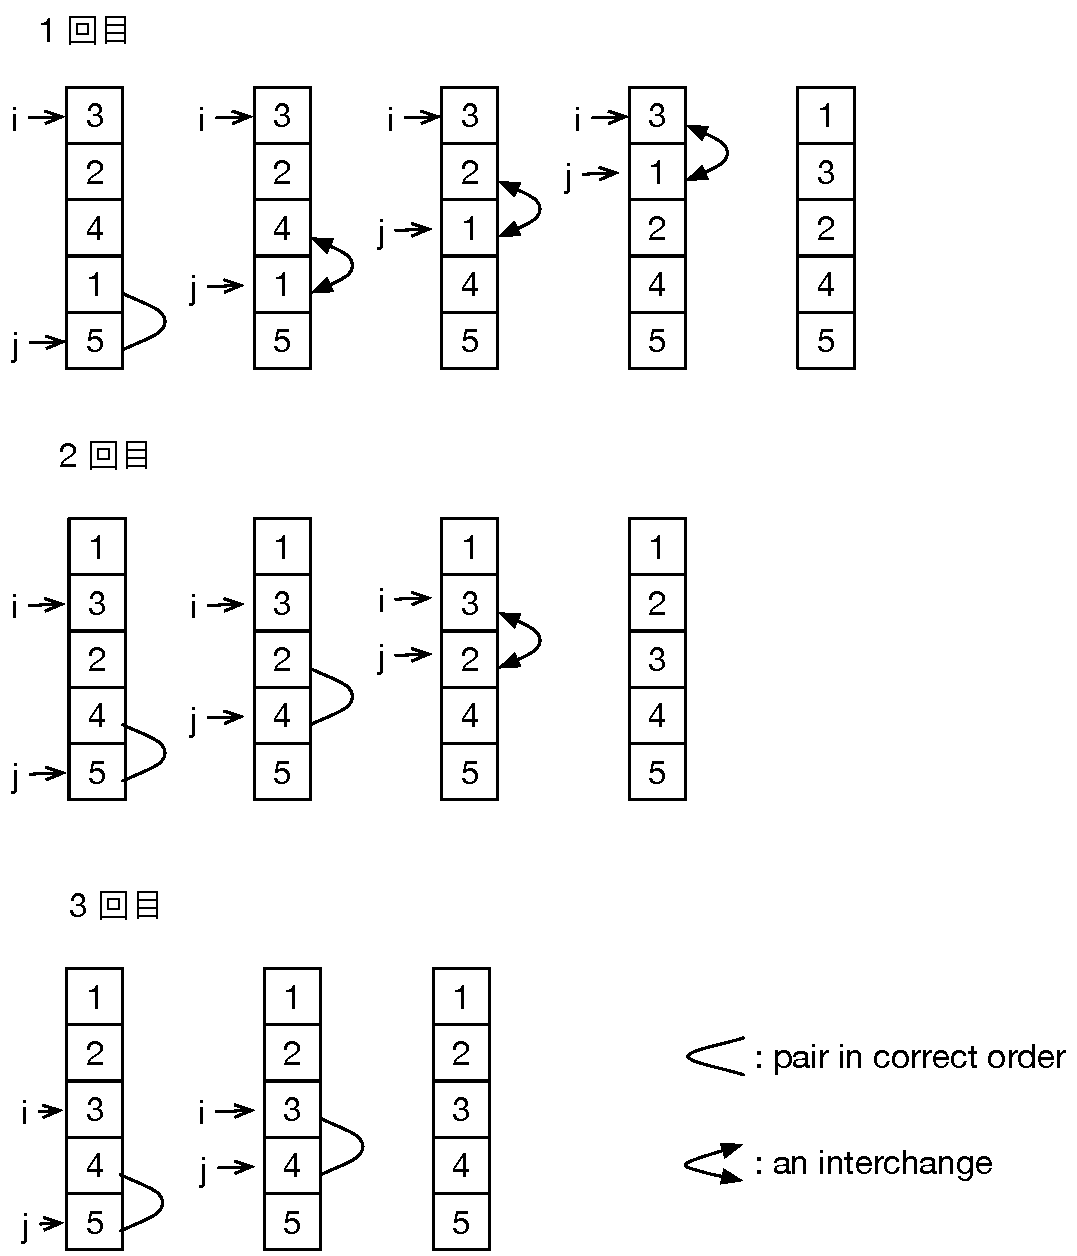
\includegraphics[scale=0.3]{./Figure/bubble_sort.pdf}
      \end{center}
    \end{column}
  \end{columns}
\end{frame}
\begin{frame}[containsverbatim,shrink]
\frametitle{Insertion Sort}
  \begin{columns}[t,onlytextwidth]
    \begin{column}{0.5\linewidth}
      \begin{lstlisting}[caption={擬似コード},label=insertion_sort]
def insertion_sort(numbers):
  for i in {2..n}:
    j=i
    while (numbers[j]<numbers[j-1]):
      numbers[j],numbers[j-1]を入替え
      j=j-1
  return(numbers)
      \end{lstlisting}
      \begin{itembox}[l]{計算量(宿題 2)}
        \begin{itemize}
\tiny
\item 配列のサイズを $n$ として \(O(n^2)\) が求められるはず
\item 宿題とするので各自で確かめてみてください
        \end{itemize}
      \end{itembox}
    \end{column}
    \begin{column}{0.55\linewidth}{様相}
      \begin{center}
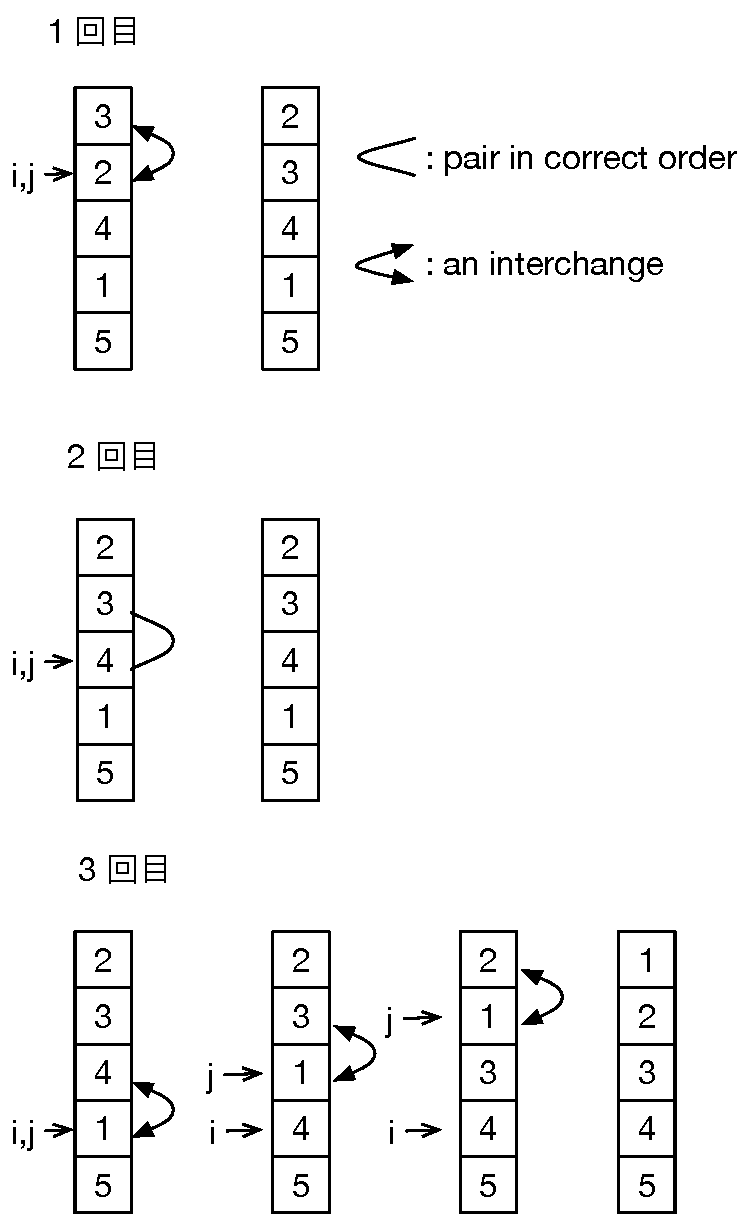
\includegraphics[scale=0.3]{./Figure/insertion_sort.pdf}
      \end{center}
    \end{column}
  \end{columns}
\end{frame}
\begin{frame}[shrink]
\frametitle{Quiz 3}
  \begin{block}{Quiz: Quick Sort}
\scriptsize
    \begin{itemize}
\item Input: 任意の長さの任意の整数の列
\item Output: 昇順に整列した列
\item \href{https://sites.google.com/presystems.xyz/elementaryCS/}{\beamerbutton{https://sites.google.com/presystems.xyz/elementaryCS/}} から sort-skeleton.py をダウンロード
\item quick sort を作成して実行時間を比較して見てください
\item 提出は sort.py としてソースコードだけ提出
    \end{itemize}
  \end{block}
  \begin{center}
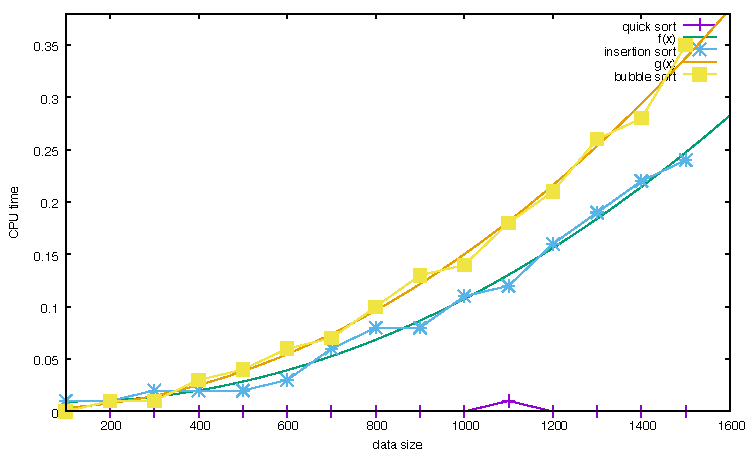
\includegraphics[scale=0.6]{./progs/sort.pdf}
  \end{center}
\end{frame}
\begin{frame}[shrink]
\frametitle{Quiz 3 の hint}
  \begin{itemize}
\scriptsize
\item Basic step: 異なる値がないときには終了
\item Recursive step:
    \begin{enumerate}
\scriptsize
\item 中間付近の値 pivot を選ぶ: findpivot()
\item pivot より小さい値を左側に,大きい値を右側に集める: partition()
\item 左側,右側でそれぞれソートする
    \end{enumerate}
  \end{itemize}
  \begin{center}
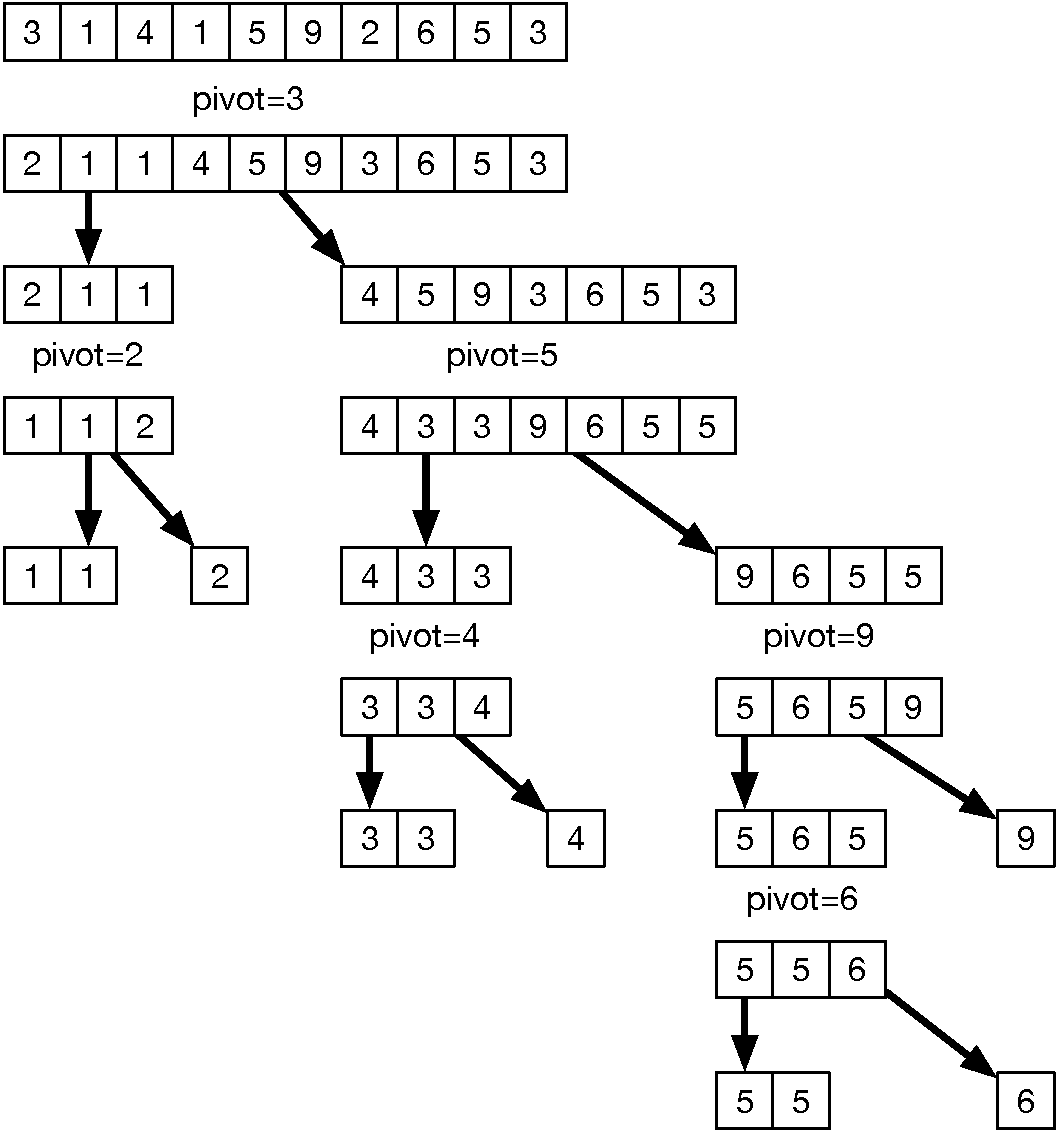
\includegraphics[scale=0.3]{./Figure/quick_sort.pdf}
  \end{center}
\end{frame}
\begin{frame}[containsverbatim, shrink]
\frametitle{Quick Sort の計算量}
  \begin{itemize}
\item 再帰関数の計算量の計算方法について見ていきます
  \end{itemize}
\vspace{-5mm}
  \begin{columns}[t,onlytextwidth]
    \begin{column}{0.45\linewidth}
      \begin{lstlisting}[caption={擬似コード},label=insertion_sort]
def partition(numbers,left,right,pivot):
  while left<=right:
    numbers[left],numbers[right] を入替え
    while (numbers[left]<pivot):
      left=left+1
    while (numbers[right]>=pivot):
      right=right-1
  return(left)
def quick_sort1(numbers,front,rear):
  pivot=findpivot(numbers,front,rear)
  if (値がすべて同じ時):
    return(numbers)
  else:
    k=partition(numbers,front,rear,numbers[pivot])
    quick_sort1(numbers,front,k-1)
    quick_sort1(numbers,k,rear)
    return(numbers)
      \end{lstlisting}
    \end{column}
    \begin{column}{0.5\linewidth}
      \begin{itembox}[l]{Best case}
        \begin{itemize}
\tiny
\item Pivot が中央のとき最適になる
\item findpivot と partition はそれぞれ $O(n)$
\item 各繰り返しでの計算回数を \(T(n)\) として
\item \(T(n)=2T(\frac{n}{2})+n\)
\item これを解いて \(T(n)=n+n\log_2(n)\)
\item したがって,全体で \(O(n\log n)\) 
        \end{itemize}
      \end{itembox}
      \begin{itembox}[l]{Worst case}
        \begin{itemize}
\tiny
\item 分割した一方が 1 個のとき最悪になる
\item 各繰り返しでの計算回数を \(T(n)\) として
\item \(T(n)=T(n-1)+T(1)+n\)
\item これを解いて \(T(n)=\frac{n^2}{2}+(T(1)+\frac{1}{2})n+T(1)\)
\item したがって,\(O(n^2)\)
        \end{itemize}
      \end{itembox}
    \end{column}
  \end{columns}
\end{frame}
\begin{frame}[containsverbatim, shrink]
\frametitle{Master Theorem}
  \begin{theorem}
漸化式が \(T(n)=aT(\frac{n}{b})+cn^d\) の形をしているときのオーダは以下のようになる
    \begin{displaymath}
T(n) = \left\{
      \begin{array}{ll}
\displaystyle
O(n^d)&\mbox{if } a<b^d \\
O(n^d\log(n))&\mbox{if } a=b^d \\
O(n^{\log_b(a)})&\mbox{if } a>b^d \\
      \end{array} \right.
    \end{displaymath}
  \end{theorem}
  \begin{itemize}
\item \(aT(\frac{n}{b})\) は大きさ $n$ の問題を \(\frac{n}{b}\) の大きさで $a$ 個に分けるという意味
\item \(cn^d\) は再帰以外の計算量の意味
  \end{itemize}
\end{frame}
%\begin{frame}[containsverbatim, shrink]
%\frametitle{ハノイの塔の場合}
%  \begin{itemize}
%\item ディスクの枚数 $n$ を入力データの大きさとして move の出現回数を数える
%  \end{itemize}
%\end{frame}

\section{Search Alogorithms}
\begin{frame}[containsverbatim,shrink]
\frametitle{宿題 3}
\framesubtitle{Search}
  \begin{itemize}
\item 余裕のある人は search algorithms に挑戦してみてください
\item Linear search と binary search の計算量を求める
\item Linear search と binary search のプログラムを作成し実行時間を比べる
\item 参考までに binary search のソースコード (search.py) を
\href{https://sites.google.com/presystems.xyz/elementaryCS/}{\beamerbutton{https://sites.google.com/presystems.xyz/elementaryCS/}} に置いておきます
\item 提出の必要はありません
  \end{itemize}
\end{frame}
%%% Shortest Path Problem
%
%\section{最適解を求める問題}
\begin{frame}
\frametitle{最短経路問題}
  \begin{itemize}
\item カーナビや乗換案内や地図で所要時間の短い経路や旅費の安い経路を案内してくれるます
\item これはグラフ理論 (Graph Theory) と呼ばれる世界の最短経路問題に帰着できます
\item 与えられた条件で最適解を求めるという問題
  \end{itemize}
  \begin{block}{余裕のある人向け quiz}
    \begin{itemize}
\item 出発地と到着地がそれぞれ与えられたとしてコストが最も小さい経路を計算するプログラムを作成してください
\item $n$ 個の node を持つとして \(O(n^2)\) のオーダで計算できます
\item グラフの表現方法を変えると \(O(n\log n)\) にできます
    \end{itemize}
  \end{block}
\end{frame}
\begin{frame}
\frametitle{グラフ理論}
  \begin{itemize}
\item グラフとはあるデータ間の関係だけに注目したモデル
\item $N$ をノードの集合 (a set of nodes), $E$ をエッジの集合 (a set of edges) としてグラフ $G$ は \((N,E)\) の対である
\item 各ノードとエッジにはラベルが付けられていて,ラベルの集合を $L$ とする
  \end{itemize}
  \begin{center}
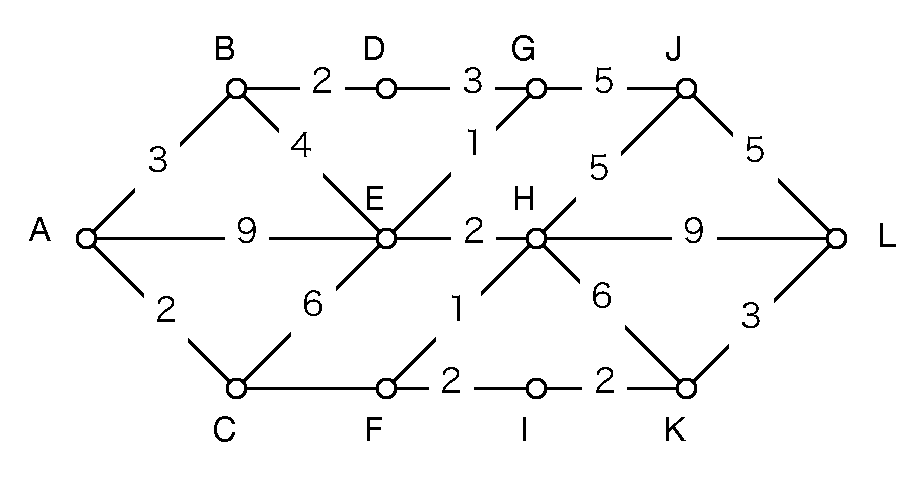
\includegraphics[scale=0.5]{./Figure/elementaryCS-2nd-figSPP.eps}
  \end{center}
\end{frame}
\begin{frame}
\frametitle{最短経路問題 (Shortest Pahts Problem)}
  \begin{itemize}
\item \(G=(N,E)\) で各エッジにコストでラベル付けし,
\item 任意の出発点が与えられたとして,他の地点に至る最小コストの経路を求める問題
  \end{itemize}
  \begin{columns}
    \begin{column}{0.3\textwidth}
      \begin{center}
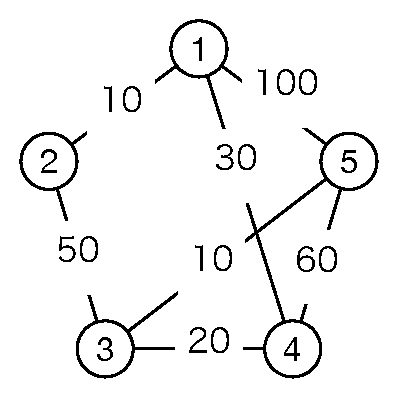
\includegraphics[scale=0.35]{./Figure/elementaryCS-2nd-figSPP-Sample.eps}
      \end{center}
    \end{column}
    \begin{column}{0.65\textwidth}
      \begin{center}
\footnotesize
        \begin{tabular}{cccccc}
S&w&D[2]&D[3]&D[4]&D[5]\\
\hline
\{1\}&\textendash&10&&30&100\\
\{1,2\}&2&10&60&30&100\\
\{1,2,4\}&4&10&50&30&90\\
\{1,2,4,3\}&3&10&50&30&60\\
\{1,2,4,3,5\}&5&10&50&30&60
        \end{tabular}
      \end{center}
    \end{column}
  \end{columns}
\end{frame}

\section{計算の複雑さのクラス}
\begin{frame}[shrink]
\frametitle{計算の複雑さのクラス}
  \begin{itemize}
\item 計算量をオーダであらわすことをみてきました
\item 計算量的に実行可能であるかという境界はどこにあるか,という疑問が出てくるのは自然なこと
\item ひとつは多項式境界 (polinomial bound) でこのクラスを P (Polynominal time) と表し,
\item もう一つを指数境界 (exponential bound) でこのクラスを NP (Non-deterministic Polynomial time) と表す.
    \begin{itemize}
\item このふたつは,決定性か非決定性かの違いや,
\item 解を得るのに全数探索しなければならないかどうかの違いとして見て取れる
    \end{itemize}
\item 有名な問題が \(\mbox{P}\neq\mbox{NP}\) かどうかという問題
  \end{itemize}
\end{frame}
